\section{Finite State Machine Realisierung}

\subsection{Realisierung von Flachen FSMs}
\begin{multicols}{2}
  \begin{itemize}
    \item Steuerkonstrukt (typischerweise mit switch-case)
          \begin{itemize}
            \item prozedural oder objektorientiert
          \end{itemize}
    \item Definition und Abarbeitung einer Tabelle
          \begin{itemize}
            \item prozedural oder objektorientiert
          \end{itemize}
    \item State Pattern (Gang of Four, GoF)
          \begin{itemize}
            \item nur objektorientiert
          \end{itemize}
    \item Generisch mit Templates
          \begin{itemize}
            \item nur mit einer Sprache, die Templates unterstützt (z.B. C++)
          \end{itemize}
    \item Alle Varianten haben wie immer sowohl Vor- als auch Nachteile
    \item Bei allen Varianten sind auch Variationen vorhanden
  \end{itemize}
\end{multicols}

\subsection{Realisierung mit Steuerkonstrukt (prozedural in C)}
\begin{figure}[h]
  \centering
  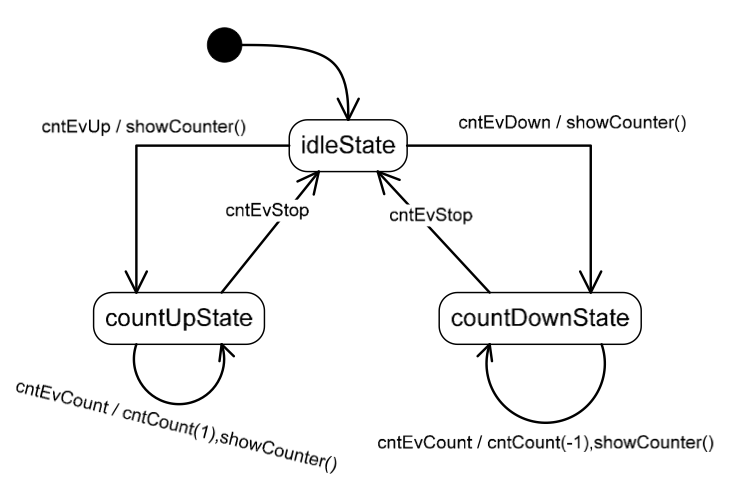
\includegraphics[scale = 0.35]{images/FSM/Up_down_counter}
\end{figure}
\begin{itemize}
  \item Zustände (States) werden in einem eunum definiert (nicht public!)
        \lstinputlisting[style=C, firstline=13, lastline=16]{snippets/Ctrl_C/counterCtrl.c}

  \item Ereignisse (Events) werden in einem enum definiert (public!)
        \lstinputlisting[style=C, firstline=12, lastline=16]{snippets/Ctrl_C/counterCtrl.h}

  \item Die FSM wird in zwei Funktionen implementiert
        \lstinputlisting[style=C, firstline=18, lastline=23]{snippets/Ctrl_C/counterCtrl.h}

  \item Der aktuelle Zustand der FSM wird in einer statischen Variablen gehalten
        \lstinputlisting[style=C, firstline=18, lastline=18]{snippets/Ctrl_C/counterCtrl.c}

\end{itemize}

\subsubsection{Vollständiger Code für prozedurales Steuerkonstrukt}
\lstinputlisting[style=C]{snippets/Ctrl_C/counterCtrl.h}
\lstinputlisting[style=C]{snippets/Ctrl_C/counterCtrl.c}
\lstinputlisting[style=C]{snippets/Ctrl_C/counter.h}
\lstinputlisting[style=C]{snippets/Ctrl_C/counter.c}
\lstinputlisting[style=C]{snippets/Ctrl_C/counterTest.c}

\subsubsection{Eigenschafteen der C-Version}
\begin{itemize}
  \item Von der FSM kann so wie sie implementiert ist nur eine Instanz vorkommen, dies kommt daher, dass der State static ist. Mögliche Lösung, State übergeben.
  \item Die Attribute der FSM (currentState) können nicht schön gekapselt werden
  \item Die Struktur ist recht einfach und kann gut erweitert werden
  \item Die Funktion cnt\_ctrlProcess() kann beliebig aufgerufen werden (z.B. aus einem periodischen Task, laufend, etc.)
  \item Die Struktur der FSM ist von aussen nicht sichtbar, der FSM werden nur die eingetretenen Events übertragen
  \item Bei exportierten Funktionen und Definitionen muss in C ein Modulkürzel vorangestellt werden (hier: cnt)
\end{itemize}


\subsection{Realisierung mit Steuerkonstrukt (Objektorientiert in
  C++)}

\begin{figure}[h]
  \centering
  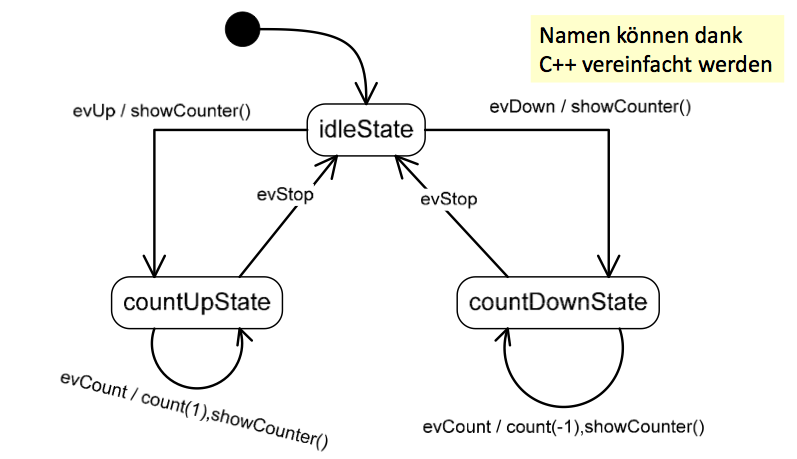
\includegraphics[scale = 0.35]{images/FSM/Up_down_counter_obj}
\end{figure}

\begin{itemize}
  \item Logisch gesehen funktioniert die objektorientierte Variante völlig identisch wie die prozedurale
  \item Dank des Klassenkonstrukts kann die FSM sauber gekapselt werden
  \item Der aktuelle Zustand der FSM (currentState) wird in einem Attribut der Klasse gehalten
        \begin{figure}[h]
          \centering
          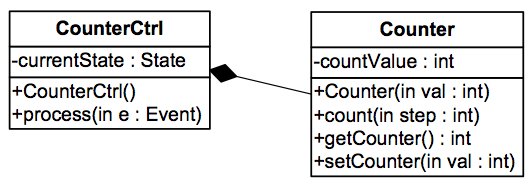
\includegraphics[scale = 0.35]{images/FSM/klasseCounter}
        \end{figure}
  \item Mehrere Instanzen derselben FSM können einfach erstellt werden
  \item Ein Modulkürzel ist nicht notwendig, da alle Namen im Kontext von Klassen definiert werden
  \item Der Code wird eleganter, eine Performanceeinbusse ist nicht vorhanden
  \item States werden im \textbf{private-Teil} der Klasse mit einem enum definiert
        \lstinputlisting[style=Cpp, firstline=26, lastline=28]{snippets/Ctrl_Cpp/counterCtrl.h}
  \item Events werden im \textbf{public-Teil} der klasse mit einem enum definiert (public, weil die Events zur Schnittstelle gehören)
        \lstinputlisting[style=Cpp, firstline=16, lastline=19]{snippets/Ctrl_Cpp/counterCtrl.h}
  \item Die FSM wird in zwei Funktionen implementiert
        \lstinputlisting[style=Cpp, firstline=20, lastline=23]{snippets/Ctrl_Cpp/counterCtrl.h}
  \item \textbf{Entry-Actions} müssen überall dort hinzugefügt werden, wo in einen neuen Zustand gewechselt wird. Üblicherweise muss die Entry-Action für einen bestimmten Zustand bei mehreren Transitionen codiert werden.
  \item \textbf{Exit-Actions} müssen überall dort hinzugefügt werden, wo ein Zustand verlassen, d.h. in einen anderen Zustand gewechselt wird. Üblicherweise muss die Exit-Action für einen bestimmten Zustand bei mehreren Transitionen codiert werden.
\end{itemize}

\subsubsection{Vollständiger Code für objektorientiertes Steuerkonstrukt}
\lstinputlisting[style=Cpp]{snippets/Ctrl_Cpp/CounterCtrl.h}
\lstinputlisting[style=Cpp]{snippets/Ctrl_Cpp/CounterCtrl.cpp}

\subsection{Realisierung mit Tabelle}
\begin{itemize}
  \item Die Tabelle kann sowohl prozedural als auch objektorientiert implementiert werden.
  \item Die objektorientierte Variante verwendet einzig die Datenkapselung. Vererbung und Polymorphismus werden nicht benötigt
  \item Die objektorientierte Variante kann klarer und schöner strukturiert implementiert werden. Im folgenden wird nur diese Variante gezeigt, die C-Version kann jedoch einfach davon abgeleitet werden
  \item Die ganze FSM ist in einer Tabelle gespeichert
  \item Die Aktionen sind als Funktionen implementiert, in der Tabelle steht der entsprechende Funktionspointer
  \item Die Abarbeitung der FSM erfolgt mit Hilfe einer \textit{Execution Engine}, die in der Tabelle "nachschaut", was zu tun ist
  \item Die Execution Engine ändert sich nicht, wenn die FSM geändert wird
  \item Das Testprogramm ist völlig unverändert
  \item Die Schnittstelle von CounterCtrl (public-Teil) ist ebenfalls identisch
  \item Die Klasse Counter ändert auch nicht
  \item Die \textbf{einzige Änderung} liegt im private-Teil der
        CounterCtrl-Klasse und natürlich in deren Implementation
  \item Alle (Tansitions-)Aktionen werden als Methoden deklariert,
        \textit{Action} wird als Funktionspointer definiert. Diese Methoden müssen
        alle mit dem Funktionspointer übereinstimmen
        \lstinputlisting[style=Cpp, firstline=33, lastline=40]{snippets/Table_Simple/CounterCtrl.h}

  \item Die Transition wird als klasseninterne Struktur deklariert. Sie besteht
        aus
        \begin{itemize}
          \item Aktueller Zustand
          \item Event
          \item Funktionspointer auf Aktionsmethode
          \item Nächster Zustand
        \end{itemize}
        fsm[] wird als statischer offener Array deklariert.
        \lstinputlisting[style=Cpp, firstline=42, lastline=49]{snippets/Table_Simple/CounterCtrl.h}

  \item Tabellendefinition in CounterCtrl.cpp (Jede Transition bildet eine Zeile)
        \begin{figure}[h]
          \centering
          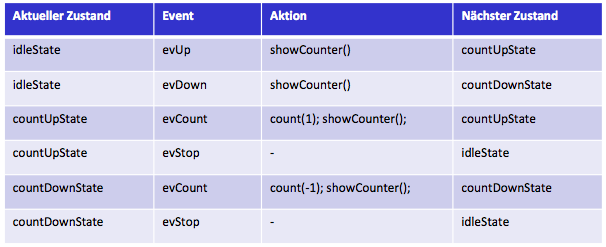
\includegraphics[scale = 0.5]{images/FSM/tabelle}
        \end{figure}
        \lstinputlisting[style=Cpp, firstline=14, lastline=22]{snippets/Table_Simple/CounterCtrl.cpp}

  \item Aufbau einer Aktionsmethode
        \lstinputlisting[style=Cpp, firstline=65, lastline=70]{snippets/Table_Simple/CounterCtrl.cpp}

  \item Performancesteigerung mit inline-Funktionen
        \begin{itemize}
          \item Die Action-Funktionen sind oft recht kurz, dennoch werden diese Funktionen immer über einen Funktionspointer aufgerufen
          \item Eine naheliegende Lösung ist, alle Action-Funktionen inline zu definieren
          \item \textbf{Leider nützt das nichts}, denn eine Funktion wird niemals inlined, wenn ein Pointer auf diese Funktion verwendet wird. Und genau das wird in der Tabelle gemacht.
        \end{itemize}

  \item Execution Engine
        \lstinputlisting[style=Cpp, firstline=30, lastline=41]{snippets/Table_Simple/CounterCtrl.cpp}

        \begin{itemize}
          \item Vor dem Aufrufen der Aktionen über den Funktionspointer müsste streng genommen überprüft werden, ob es sich um einen gültigen Pointer handelt $\rightarrow$ aus Performancegründen wird darauf verzichtet
          \item Voraussetzung dafür ist, dass in der Tabelle immer ein gültiger Pointer auf eine Memberfukntion vorhanden ist. Wenn nichts zu tun ist, soll ein Pointer auf eine leere Funktion eingesetzt werden (im Beispiel der Pointer \&counterCtrl::actionDoNothing)
          \item Da sich die Tabelle und die Execution Engine in derselben Datei befinden, ist dieses Vorgehen unproblematisch, bzw. sogar die bevorzugte Variante
        \end{itemize}

  \item Erweiterungsmöglichkeit: Wenn der Zustandsübergang nicht nur durch einen Event, sondern eine komplexe Prüfung (Event und Guard) ausgelöst wird, dann könnte der Eventeintrag in der Tabelle durch einen weiteren Funktionspointer auf eine Checkfunktion ersetzt werden
        \lstinputlisting[style=Cpp, firstline=33, lastline=33]{snippets/Table/CounterCtrl.h}
        \lstinputlisting[style=Cpp, firstline=36, lastline=36]{snippets/Table/CounterCtrl.h}
        \lstinputlisting[style=Cpp, firstline=51, lastline=57]{snippets/Table/CounterCtrl.h}
\end{itemize}

\subsubsection{Vollständiger Code für Tabellen-Realisation}
\lstinputlisting[style=Cpp]{snippets/Table/CounterCtrl.h}
\lstinputlisting[style=Cpp]{snippets/Table/CounterCtrl.cpp}

\subsection{Realisierung mit State Pattern}
\begin{itemize}
  \item Das Prinzip besteht aus einer abstrakten State-Basisklasse. Pro Zustand
        muss eine eigene Klasse definiert werden, die von dieser abstrakten
        Basisklasse erbt.
  \item Die Realisierung nutzt das Polymorphismus-Konzept, jede konkrete
        State-Klasse ist ein \textit{Singleton}
  \item Statt lange switch-case-if-Konstrukte wird beim State Pattern ein
        bestimmter Zustand vollständig in einer eigenen Klasse realisiert. Die Logik
        wird somit aufgeteilt.
  \item \textbf{Context} definiert die interessierenden Schnittstellen für
        Clients, unterhält eine Instanz einer konkreten Unterklasse von State, die den
        aktuellen Zustand definiert, bzw. repräsentiert
  \item \textbf{State} definiert eine schnittstelle zur FMS in Form einer
        abstrakten Klasse
  \item \textbf{ConcreteStateX Unterklassen} jede Unterklasse implementiert
        genau einen Zustand (ist Singleton)
        \begin{figure}[h]
          \centering
          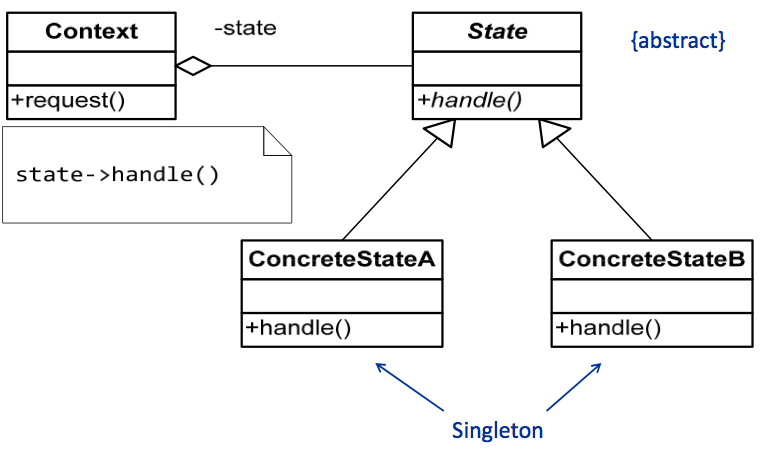
\includegraphics[scale = 0.3]{images/FSM/state_pattern}
        \end{figure}
  \item Das State Pattern definiert die Zuständigkeit der state Transition nicht
  \item Die Transitionen könnten in der Context-Klasse definiert werden. Der
        Nachteil dieser Variante ist, dass dort zentral sehr viel Intelligenz vorhanden
        sein müsste. Da diese Klasse auch den Zugriff zur Aussenwelt darstellt, sollte
        sie möglichst schlank sein.
  \item Die bessere Variante ist, wenn die State-Klassen auch gleich ihre
        Transitionen realisieren. Diese Variante wird oft mittels friend-Deklaration
        realisiert, was jedoch nicht nötig ist
  \item Schnittstelle zur State Machine; CounterCtrl ist die Context-Klasse; process() entspricht request()
\end{itemize}

\begin{center}
  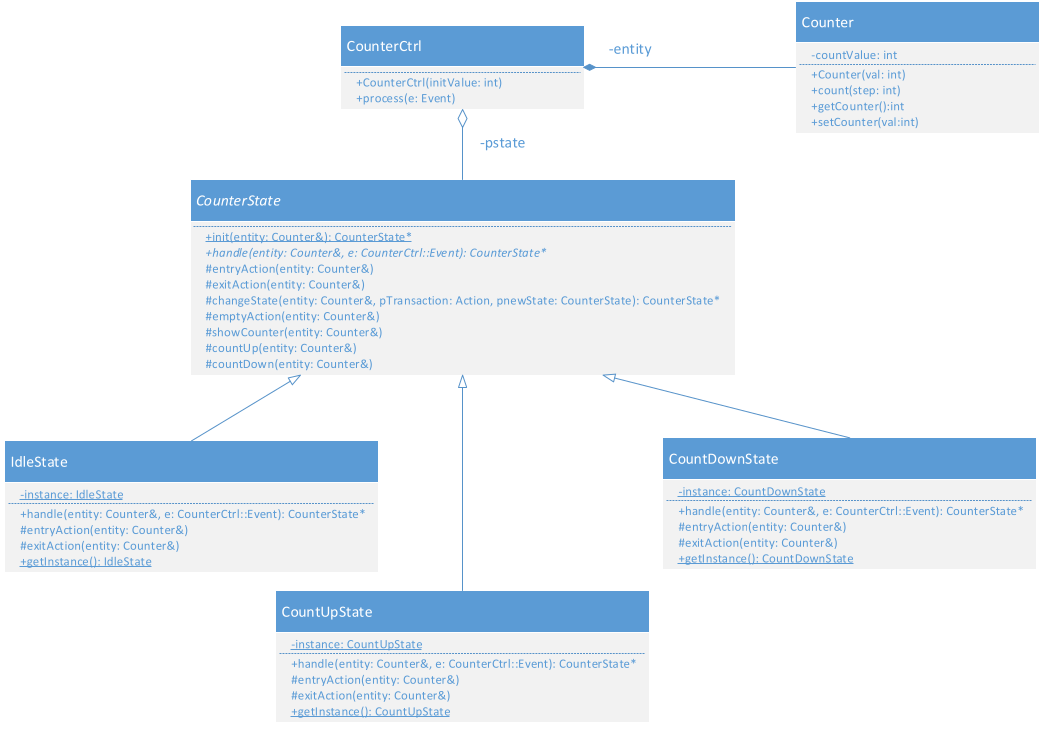
\includegraphics[width=0.7\linewidth]{./images/FSM/klassendiagramm}
\end{center}

\begin{itemize}
  \item counterCtrl.h : Schnittstelle zur FSM
        \lstinputlisting[style=Cpp]{snippets/Pattern_Action/CounterCtrl.h}

  \item counterCtrl.cpp
        \lstinputlisting[style=Cpp]{snippets/Pattern_Action/CounterCtrl.cpp}

  \item class CounterState: Interface
        \lstinputlisting[style=Cpp]{snippets/Pattern_Action/CounterState.h}
        \begin{itemize}
          \item CounterState::changeState(...)
                \begin{itemize}
                  \item Diese Funktion könnte für diese Anwendung auch wegoptimiert werden, aus Kompatibilitätsgründen für (noch folgende) Erweiterungen soll sie jedoch beibehalten werden
                \end{itemize}
          \item CountUpState::getInstance() ist eine statische Funktion mit class scope. Sie ist zusammen mit instance charakteristisch für das Singleton
          \item CountUpState::handle() ist spezifisch für diesen State zu implementieren
          \item CountUpState::CountUpState ist der private Default Ctor der verhindert, dass von dieser Klasse Objekte erzeugt werden können
          \item CountUpState::entryAction() und CountUpState::exitAction() müssen nur dann deklariert und überschrieben werden, wenn es wirklich etwas Spezifisches zu tun gibt, andernfalls wird die Default-Implementation der Basisklasse genommen
        \end{itemize}
  \item class CounterState: Implementation
        \lstinputlisting[style=Cpp]{snippets/Pattern_Action/CounterState.cpp}
\end{itemize}

\subsection{Realisierung von hierarchischen State Machines}
\begin{itemize}
  \item Toolunterstützung
        \begin{itemize}
          \item IBM Rhapsody, MathWorks Matlab/Simulink mit RT Workbench, u.a.
        \end{itemize}
  \item QP-Framwork
        \begin{itemize}
          \item Framwork für Ausführung mit oder ohne Betriebssystem
          \item Ressourcenbedarf: 1kB RAM, 10kB ROM
          \item Targets: Cortex-M4
          \item QP-nano für kleine Controller (z.B. MSP430, 8051, PIC, AVR)
          \item Ressourcenbedarf QP-nano: 100 Bytes RAM, 2kB ROM
        \end{itemize}
\end{itemize}

\newpage
